\chapter{Technological Foundation}
\label{chap:technological-foundation}
\epigraph{``I became convinced from the start that the notion of a state and a transition to a new state was fundamental to their thinking about the system.''}{\textit{David Harel}}
\noindent
Crossing the interdisciplinary boundaries between programming and psychology needs the definition of the technical concepts that are referenced.
For example knowing what is meant by \emph{state} and \emph{transition} in David Harel's above-mentioned psychological discovery is necessary to understand why this might impact the way people think about systems. 
As stated by \textcite{schraube_ich_2012}, the interaction between a person's psyche and technology is always bidirectional, we get shaped by technology the same way we shape it.

\section{Characteristics of Software Development Processes}
\todo{that's new}
\label{sec:characteristics-of-software-development-processes}
Upon answering the question on how communication in software development processes can be improved using technology, it is important to define these processes, take a quick look at the history and examine the difficulties of changing requirements.

The complex process of software development involves a lot of tasks, stakeholders and uncertainties \autocite{mayr_projekt_2005}.
Being able to plan, organize and control this process, different paradigms of organizing the process of software development were established and improved.
Independent of the software development paradigm, six main phases can be identified, namely: \emph{requirements analysis}, \emph{specification}, \emph{design}, \emph{implementation}, \emph{testing} and \emph{maintenance} \autocite{harel_statecharts:_1987}.
Somehow those phases have to be completed in that order, albeit the paradigms differ in the way the phases are went through, 
The most notable differences are the flexibility in adapting to changing requirements, customer communication, the way phase transitions are handled, how fast the project iterates and how often intermediate results are delivered \autocite{mayr_projekt_2005}.

\subsection{Traditional Paradigms vs. Agile Paradigms}
\todo{that's new}
\label{sub:traditional-vs-agile}
As described in \textcite{mayr_projekt_2005}, the evolution of software development paradigms underwent a lot of change.
Over time the characteristics changed from rigorous (traditional, heavy and stable) to agile (modern, lean, fragile), with the agile movement based on \textcite{fowler_agile_2000} as the current status quo \autocite{ousterhout_philosophy_2018}.
In comparison to the documentation-heavy traditional paradigms, agile paradigms got rid of documentation overhead, heavily rely on prototyping and follow an iterative-incremental model \autocite{mayr_projekt_2005}.
This iterative-incremental model is characterized by short consecutive development cycles and a high frequency in delivering intermediate products, thus staying in close contact with the customer, making sure that the right product is delivered and requirements are understood correctly \autocite{mayr_projekt_2005}.
Dispensing long requirement analysis and specification phases in favor of a short time to market affects software architecture and design, subsequently complicating the creation of well-architectured, solid software.
\textcite{ousterhout_philosophy_2018} introduces the terms \emph{tactical programming} and \emph{strategic programming}.
While the main focus of tactical programming is to create something that works, the focus of strategic programming is to create something that lasts.
In the end this is a business decision, but the effects it has on software development have a huge impact regarding the design of stable, well-constructed systems \autocite{ousterhout_philosophy_2018}.

\subsection{Requirements Analysis and Changing Requirements}
\label{sub:requirements-analysis}
Requirements are properties that have to be fulfilled by a system \autocite{mayr_projekt_2005}.
Requirements analysis is the process of understanding what the customer needs and translating these to a specification upon which the software program can be built.
It is necessary that these identified requirements can be validated and verified.

As stated in \textcite{mayr_projekt_2005} the difficulties of requirements analysis are often underestimated.
Two of these are of high importance for this thesis.
Requirements analysis is a human-centered communication process.
Analysts have to understand the customer's domain, excel at communication with various stakeholders and create a form of specification that is understood by all participants as well as traceable from the origin of a requirement into the finished product.
As \textcite[265]{curtis_psychology_1990} discovered: ``That is, many projects spen[d] tremendous time rediscovering information that, in many cases, had already been generated by customers, but not transmitted.''
Changing requirements caused by the customer, by competitors or by new market innovations are another big problem for requirements analysis.
As stated by \textcite{mayr_projekt_2005}, requirements analysts' methods and notations should favor an easy way of adapting new and changing requirements.

Even if the analysts' methods can adapt to changing requirements, the difficulty of communication still exists and gets intensified by rapidly changing requirements.
More closely aligning the methods and notations of analysts to those used in the implementation phase can reduce these costly communication problems.
According to Peter Naur the designer's (analyst's in this case) job is not to pass along ``the design'' but to pass on ``the theories'' driving the design \autocite{naur_programming_1985} preventing documentation being an ``auxiliary, secondary product.''

\textcite{leveson_experiences_1991} report an interesting experience on requirements specification while working on an aircraft collision avoidance system called \emph{TCAS II}.
After realizing that the \emph{minimal operational standards} document (MOPS) initially created specified the behavior too loosely, an industry/government alliance started working on a more detailed specification in English.
At the same time \textcite{leveson_experiences_1991} started working on a formal specification.
After only one year the English specification was dropped in favor of the formal specification, because of not being able to handle the complexity in a correct way.
Admittedly adopting the formal specification brought its problems as well.
There is a sweet spot in requirements specification described by \textcite{leveson_experiences_1991}: ``The specification must be formal enough [...] to use as a basis for a safety analysis. It must also be readable enough for noncomputer experts to read and review and be usable for both building and certifying [...] systems.''

\subsection{Insights from Psychology}
\label{sub:insights-from-psychology}
\citeauthor{kitchenham_research_1990} identified the uniqueness of the software development process in the following way: ``Closer inspection of the software production process suggests that it is an engineering discipline like any other engineering discipline. It is not as mature as electrical or chemical engineering or even agriculture. Nonetheless, it is \emph{not} an art form. Before software engineering can mature as an engineering discipline, practitioners need a better understanding of the process by which software is created in response to a demand and of the risks and errors which are associated with the process.'' \autocite[274]{kitchenham_research_1990}, conducting that the major difference to other engineering disciplines is the missing maturity and empirical knowledge.

While most software development process paradigms originate in economics, the layered behavioral model (\cref{fig:layered-behavioural-model}) of software development \autocite{curtis_psychology_1990} emphasizes the cognitive, social and organizational processes.
\begin{figure}[h]
\centering
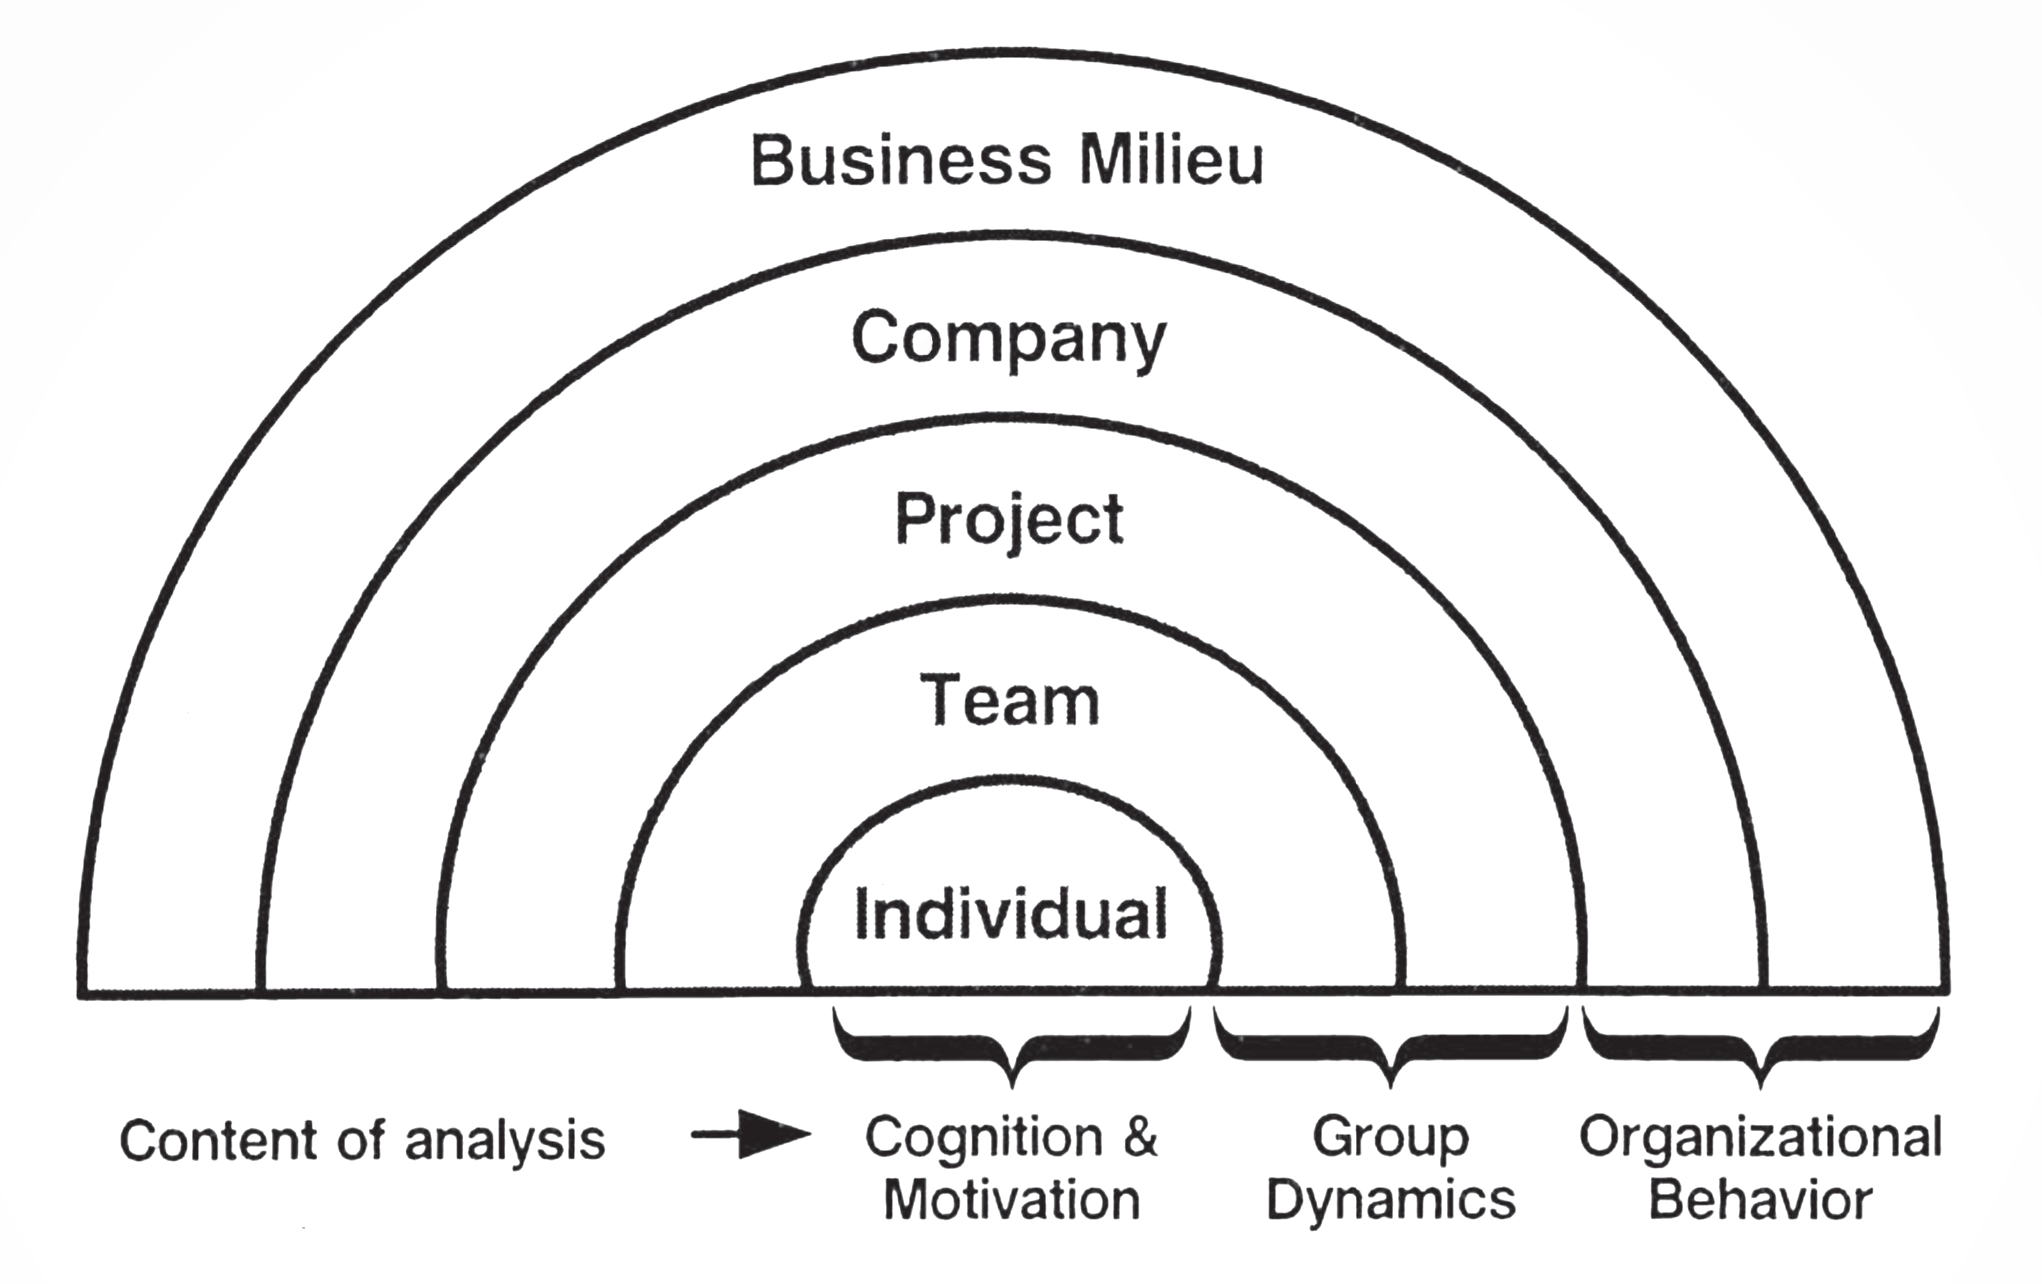
\includegraphics[width=0.7\textwidth]{layered-behavioural-model}
\caption{Layered Behavioral Model of Software Development}
\label{fig:layered-behavioural-model}
\end{figure}
They stated that ``the layered behavioral model focuses on the behavior of the humans creating the artifact, rather than on the evolutionary behavior of the artifact through its developmental stages'' \autocite[254]{curtis_psychology_1990}.
Confirming Curtis' findings, Gerald M. Weinberg already presented empirical studies about ``Programming as a Social Activity'' in 1971 \autocite{weinberg_psychology_1971}.
His studies also focus on the much understated social aspects of programming while most of the focus is put on tools for helping the individual developer, and forgetting about group, team and project communication.

Regarding communication, \textcite{curtis_psychology_1990} introduce the concept of a \emph{boundary spanner}.
During their empirical studies about the social aspects of psychology of programming they identified: ``Boundary spanners translated information from a form used by one team into a form that could be used by other teams'' \autocite[264]{curtis_psychology_1990}.
They become ``hubs for information'' \autocite[264]{curtis_psychology_1990} introducing the problem of implicit hidden knowledge that is not documented.
Regarding the title of this thesis, boundary spanners ``align mental models and models used in software development'', they transmit and translate knowledge.
The goal is not to replace boundary spanners, but merely inviting more and more people in the software development process to take part in transferring knowledge, spanning boundaries and talking about the same things.


\section{Statecharts}
\label{sec:statecharts}
Invented in 1983 by David Harel, statecharts are ``visual formalism for complex systems'' \autocite{harel_statecharts:_1987}.
While working on avionic systems for the Israeli Air Force, David Harel was asked to help taming the complexity of reactive systems.
A reactive system is dominated by its ``[...] reactivity; its event-driven, control-driven, event-response nature, often including strict time constraints, and often exhibiting a great deal of parallelism. A typical reactive system is not particularly data intensive or calculation intensive'' \autocite{harel_statecharts_2007}.
Reading this pretty narrow technical definition of a reactive system one might question the relevance of statecharts in everyday software.
Ian Horrocks provides an answer to this question by specifying the \emph{event-action paradigm} \autocite{horrocks_constructing_1999}.
User Interfaces are event-driven, they present screens with data and wait for user interactions.
Based on these they react, thus fulfilling all the requirements for a reactive system.
And because every software that is interacted with has some kind of user interface, all these programs can utilize statecharts as a way of handling state.

Describing a visual notation with words is contradictory, so let's take a look at \cref{fig:statecharts-example} taken out of the original paper introducing statecharts \autocite{harel_statecharts:_1987}.
This statechart describes part of the behavior of a digital wristwatch.
The rounded rectangles describe states the system can be in and the labeled arrows between these describe the state transitions.
Basically a statechart is an enhanced mixture between state diagrams and flow charts.
This also explains where the name comes from, according to David Harel the term \emph{statecharts} was the only unused combination of ``'state' or 'flow' with 'chart' and 'diagram''' in 1983.

\begin{figure}[h]
\centering
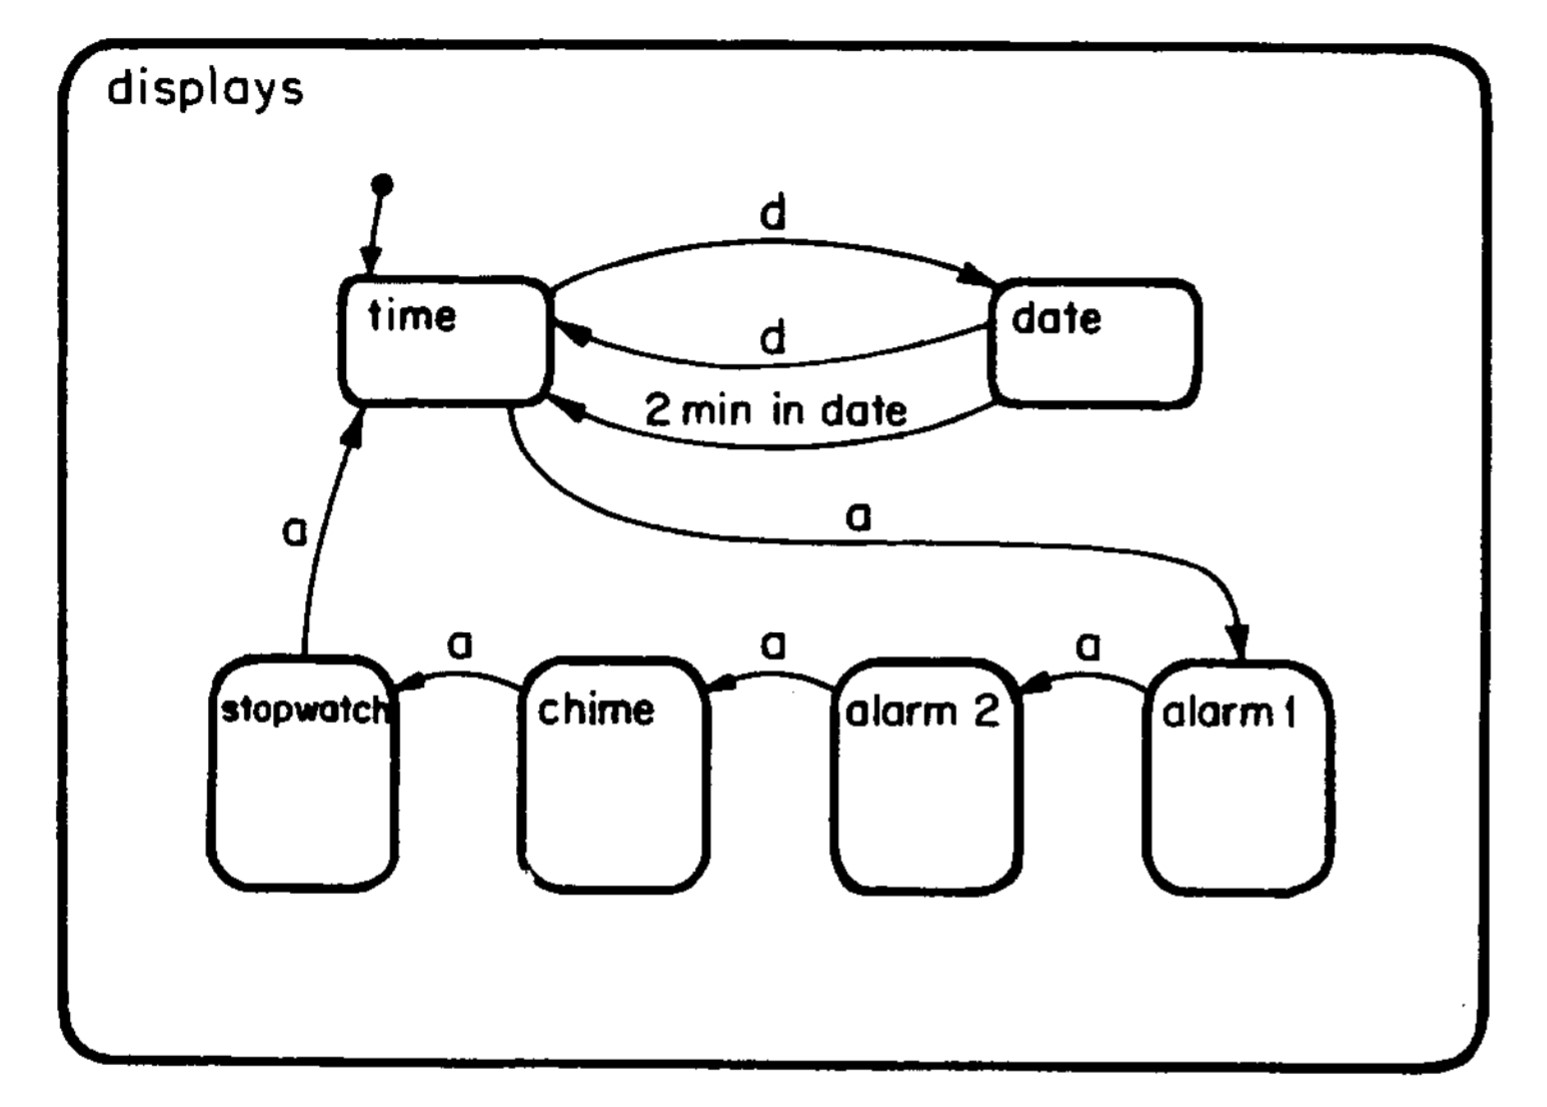
\includegraphics[width=0.8\textwidth]{small-statechart-example}
\caption{Example Statechart of a Digital Wristwatch Interface}
\label{fig:statecharts-example}
\end{figure}

As T.G.R. Green defines in \textcite[3]{green_pictures_1982} ``A \emph{program} is a succinct description of a temporal process.''
Martin Glinz describes why statecharts perfectly fit Green's definition of a program: ``Naturally, statechart models will concentrate on requirements concerning dynamic system behavior and interaction'' \autocite[1]{glinz_statecharts_2002}.
Taking a look at \cref{fig:statecharts-example} this statechart transmits this information in the following way:
\begin{itemize}
    \item The outermost box \emph{displays} is a compound state containing multiple sub-states such as \emph{time}, \emph{data}, \emph{alarm 1} and so on. In statecharts a compound state is defined by having multiple sub-states with exactly one being active at a certain point in time.
    \item The arrow originating in a black dot leading into \emph{time} specifies that this state is the initial active state of \emph{displays}.
    \item The labels \emph{d} and \emph{a} name events that can happen in a the system. In this particular example by David Harel the digital wrist watch contains four buttons, that upon pressing raise the events \emph{a}, \emph{b}, \emph{c} and \emph{d}.
    \item The arrows labeled \emph{d} between \emph{time} and \emph{date} can be translated to a toggle functionality between the time and display states of the watch.
    \item The arrow labeled with \emph{2 min in date} follows exactly its description. If the state \emph{date} has been active for two minutes and no event occurred the state \emph{time} is automatically entered.
    \item If the system is in state \emph{time} and the event \emph{a} occurs it will transition to \emph{alarm 1}, on another press of \emph{a} into state \emph{alarm 2} and so on.
\end{itemize}

One of the most important properties of statecharts in comparison to textual source code is the obviousness of valid and invalid transitions.
Users of the statechart can immediately conclude which events are possible in which state.
Another property of statecharts is that events not allowed in the currently active state are simply ignored instead of causing errors, thus leading to more robust and less faulty programs \autocite{horrocks_constructing_1999}.
For a full overview of the available features of statecharts please refer to \textcite{harel_statecharts:_1987}.

\subsection{The Goals Behind}
\label{sub:goals-behind-statecharts}
In \citeyear{harel_statecharts_2007}, David Harel published his personal story behind statecharts titled ``Statecharts in the Making: A Personal Account'' \autocite{harel_statecharts_2007}.
In this paper he talks about his psychological ideas and observations during the development of statecharts in the eighties.
Apart from creating a \emph{visual formalism} for reactive systems, he wanted to create a notation for \emph{model-based development} (which became really popular with the Unified Modeling Language [\textcite{cook_unified_2017}]) and an executable model where the behavior ``can and should be executed just like [with] conventional computer programs [...]'' \autocite[1]{harel_statecharts_2007}.
This technical goals lay the foundation for two of his greater goals that can be attributed to social psychology \autocite[3--4]{harel_statecharts_2007}:
\begin{itemize}
    \item ``The goal was to try to find, or to invent for these experts, a means for simply saying what they seemed to have had in their minds anyway.''
    \item ``The goal was to find a way to help take the information that was present collectively in their heads and put it on paper, so to speak, in a fashion that was both well organized and accurate.''
\end{itemize}

The above mentioned \emph{executability} is another fundamental idea of statecharts \autocite[7]{harel_modeling_1998}, because of the simulation aspect taking a lot of cognitive load off the developer.
Back in the eighties executable models weren't the standard, because the graphics and input capabilities of computers were not comparable to the ones used today, but even then David Harel imagined ``[...] graphical workstations with large (blackboard size?) displays of fantastic resolution [...]'' \autocite[272]{harel_statecharts:_1987}.
More than 30 years later, devices like the Microsoft Surface Hub\footnote{\url{https://www.microsoft.com/en-us/surface/business/surface-hub-2}} exist that perfectly match this description.
Combined with Bret Victor's ideas of instant code executability \autocite{victor_inventing_2012} this could be the perfect match for an interactive development environment based on statecharts.

\subsection{Aligning Thoughts with Fractal Architectures}
\label{sub:aligning-thoughts-with-fractal-architectures}
Comparing different approaches to user interface development, André Staltz coined the term \emph{fractal architecture} as ``[an] architecture is said to be fractal if subcomponents are structured in the same way as the whole is'' \autocite{staltz_unidirectional_2015}.
Fractals are a mathematical concept of geometric figures that appear the same at different levels.

As described earlier, statecharts feature the concept of compound states, wherein states can be nested inside each other.
This property perfectly maps to ``geometric figures that appear the same at different levels'' and André Staltz's definition of fractal architectures.
This state nesting allows to refine the behavior of a certain state by adding sub-states and thus adapting to new requirements without breaking others \autocite{harel_statecharts:_1987}.
\textcite{leveson_experiences_1991} discuss the two main strategies of transforming requirements into software: \emph{top-down} and \emph{bottom-up}.
The top-down strategy is based on top-down refinement where requirements are deconstructed one by one, starting from the most abstract one transitioning down the tree of requirements.
Unfortunately, this process only works for experts possessing a huge knowledge in software design and the problem domain.
The bottom-up strategy, on the other hand, is characterized by less upfront thoughts about design and immediately starting with the implementation of requirements at a very detailed level.
A major problem using this approach is that a well designed software architecture is nearly impossible to reach, especially as applications get larger \autocite{horrocks_constructing_1999}.
As stated in \textcite{leveson_experiences_1991}, programmers constantly switch between those two strategies while developing software.

This is exactly the point where the fractal nature of statecharts can be aligned with the characteristics of programming.
States itself can be nested (\emph{bottom-up}) as well as refined using sub-states (\emph{top-down}), directly resembling the composition and decomposition of requirements as shown by \textcite{leveson_experiences_1991}.
\textcite{glinz_statecharts_2002} already started research in the direction of transforming requirements into statecharts, but only from a technical and not from a psychological perspective.


\section{Hole-Driven Development}
\label{sec:hole-driven-development}
The term \emph{Hole-Driven Development} is not yet scientifically defined, but based on other programming concepts like \emph{Type-Driven Development} \autocite{brady_type-driven_2017} or \emph{Test-Driven Development} \autocite{mccracken_digital_1957}.
The main idea stems from the \emph{Agda} programming language\footnote{\url{https://wiki.portal.chalmers.se/agda/pmwiki.php}} where \emph{holes} are called \emph{goals}.
Apart from Agda, other languages such as Haskell\footnote{\url{https://www.haskell.org/}} and Idris\footnote{\url{https://www.idris-lang.org/}} feature the concept of holes.
The common properties of those languages is their functional nature and a very sophisticated type system.
These two aspects lay the foundation for Hole-Driven Development as currently understood.

Simply said, a \emph{hole} declares a missing part in an application.
\textcite{gamari_haskell_2019} contains the up to now most comprehensive description of the concept of holes, while \textcite{brady_type-driven_2017} created the example shown in the following section.

\subsection{Example in Idris}
\label{sub:hole-driven-development-in-idris}
The Idris program in \cref{fig:idris-program-hole} demonstrates the simplest possible hole.
In Line \verb|2| the function \verb|main| is defined that should print something (using the standard library function \verb|putStrLn|) to the console.
The ``hole'' part of this program is \verb|?greeting|.
Signaling a hole, the question mark tells the Idris compiler that something in this program is missing that the developer didn't specify yet.
The syntax using a question mark resembles a question to the compiler.

\begin{figure}[h!]
\begin{lstlisting}[language=Haskell,firstnumber=1]
main : IO ()
main = putStrLn ?greeting
\end{lstlisting}
\caption{Hole-Driven Development in Idris}
\label{fig:idris-program-hole}
\end{figure}

Edwin Brady coined the phrase ``the compiler as your lab assistant'' \autocite{brady_type-driven_2017}.
His imagination of a compiler is one of a counterpart one interacts or pair-programs with.
One tells the compiler all the things that are currently in ones mind and as a reward one can ask questions and the compiler will try to answer those based on the knowledge already provided.
In terms of psychology, this is a pretty human way of interacting with the computer.

A practical example of this ideas looks like the following output of Idris' interactive command line interface.
Using \verb|:t greeting| one can ask the compiler for the type of the hole ``greeting''.
As an answer one gets \verb|greeting : String| which signals that the missing value is of type String, or in a non-technical terminus simply a text to complete the program definition.

\begin{verbatim}
*Hello> :t greeting
--------------------------------------
greeting : String
\end{verbatim}

In contrast to the previous example, if you just try to use \verb|greeting|, the Idris compiler tells you that you have a hole in your program labeled \emph{greeting} of type String.
This shows the communication process Edwin Brady talks about.

\begin{verbatim}
*Hello> greeting
?greeting : String
\end{verbatim}

``Holes allow you to develop programs \emph{incrementally}, writing the parts you know and asking the machine to help you [...]'' \autocite[21]{brady_type-driven_2017}.
Stepping a little bit back and comparing this way of developing software to how software development processes evolved (see \cref{sub:traditional-vs-agile}), the similarities are unmistakable.
Let's take a look at how holes are simulated in programming languages that don't support this feature natively before we get to psychological observations that were already discovered in the field of psychology of programming.

\subsection{Simulating Holes}
In languages that do not provide the feature of typed holes, programmers tend to come up with alternative solutions to holes without knowing of their existence.
Psychological research (see \cref{sub:incomplete-thoughts}) indicates that the process of creating these holes is so natural to the thought process that even within languages without the concept of holes, developers find a way of expressing those.
There are mainly two ways of simulating holes:
\begin{enumerate}
\item One might throw exceptions such as \verb|NotImplementedException|, as documented in \textcite{microsoft_notimplementedexception_2020}, to signal that a feature is not yet implemented.
\item Comments are another common way of deferring development of a particular method or feature, marking the comment as a ``hole'' prefixing it with \verb|TODO:|. E.\,g. in C\#\footnote{\url{https://docs.microsoft.com/en-us/dotnet/csharp/}} this looks like \verb|// TODO: Load state from previously suspended application|. Interactive development environments are able to parse this information and provide an overview of to-dos as shown in \textcite{hogensen_use_2019}.
\end{enumerate}
These two concepts might look like sufficient surrogates at first, so what are the differences to real holes?
\begin{itemize}
    \item The previously described interaction with the compiler is missing completely.
    \item By using exceptions the program crashes at run-time, which results in buggy software. Additionally, there is no real overview of all the simulated holes. One has to do a text-based search for the exception name.
    \item Utilizing comments doesn't result in the program crashing, rather not adhering to the specifications without any note at run-time. This might lead to incorrectly behaving software.
    \item Both approaches act like a ``do-it-later'' approach, without actively reminding the developer at a later time.
\end{itemize}

\subsection{Incomplete Thoughts}
\label{sub:incomplete-thoughts}
In the meta-analysis \citetitle{visser_expert_1990} \citeauthor{visser_expert_1990} conducted in \citeyear{visser_expert_1990} collected thinking processes and strategies of expert programmers \autocite{visser_expert_1990}.
Comparing breadth-first and depth-first design methodologies, they found out that expert developers vary in their usage and most of the time combine both strategies.
One commonality was the observation that the developers under research were observed making ``notes to themselves'' \autocite[241]{visser_expert_1990}.
Experts usually excel at maintaining relevant information in memory, nevertheless this memory capacity is limited and working on one problem might relate to other problems until there is not enough capacity left and they start taking those notes.
They conclude that ``[...] before introducing the constraints of actual programming languages, experts very often use[d] a personal pseudo-code'' \autocite[242]{visser_expert_1990}.

Combining this research, it seems plausible that real holes enhanced with comments could lead to a programming language that lets developers specify the already thought-out ideas in executable source code while still letting them express their ideas in written natural language with the advantage of the programming environment caring about their ideas.


% The internal model is iteratively finetuned during requirements specification development to mimic our understanding of the process with sufficient detail to achieve the desired control performance.